\documentclass[10pt, a4paper]{article}
\usepackage[a4paper]{geometry}
\usepackage[utf8]{inputenc}
\usepackage{amsmath,amsthm,amssymb,xfrac}
\usepackage{fancyhdr}
\usepackage[hungarian]{babel}
\usepackage{graphicx}
\usepackage{float}
\usepackage{comment}
\usepackage{siunitx}
\usepackage{hyperref}
\usepackage{siunitx}
\usepackage{natbib}
\usepackage{empheq}
\usepackage{wrapfig}
\usepackage{chngcntr}
\usepackage{physics}
\usepackage{mathtools}
\counterwithin{figure}{section}
\usepackage{titlesec}
\usepackage{dsfont}
\usepackage{pdfpages}
\usepackage{t1enc}
\usepackage{tabto}
\graphicspath{ {./images/} }


\newcommand{\N}{\mathbb{N}}
\newcommand{\Z}{\mathbb{Z}}
\newcommand{\R}{\mathbb{R}}
\newcommand{\Q}{\mathbb{Q}}

\newcommand{\adat}{\begin{trivlist}\item[\hskip \labelsep {\bfseries 
			{Adatok:}}]\end{trivlist}}
\newcommand{\egy}{\begin{trivlist}\item[\hskip \labelsep {\bfseries 
			{1. Feladat:}}]\end{trivlist}}
\newcommand{\ketto}{\begin{trivlist}\item[\hskip \labelsep {\bfseries 
			{2. Feladat:}}]\end{trivlist}}
\newcommand{\harom}{\begin{trivlist}\item[\hskip \labelsep {\bfseries 
			{3. Feladat:}}]\end{trivlist}}
\newcommand{\negy}{\begin{trivlist}\item[\hskip \labelsep {\bfseries 
			{4. Feladat:}}]\end{trivlist}}		
\newcommand{\ot}{\begin{trivlist}\item[\hskip \labelsep {\bfseries 
			{5. Feladat:}}]\end{trivlist}}
\newcommand{\ellenorzes}{\begin{trivlist}\item[\hskip \labelsep {\bfseries 
			{Ellenőrzés:}}]\end{trivlist}}
\newcommand{\hatodik}{\begin{trivlist}\item[\hskip \labelsep {\bfseries 
			{6. Feladat:}}]\end{trivlist}}
\newcommand{\het}{\begin{trivlist}\item[\hskip \labelsep {\bfseries 
			{7. Feladat:}}]\end{trivlist}}
\newcommand{\into}[2]{(#1)$\xrightarrow{}$(#2):}
\newcommand{\knm}{\;\mathrm{\left[kNm\right]}}
\newcommand{\kn}{\;\mathrm{\left[kN\right]}}
\newcommand{\meter}{\mathrm{\left[m\right]}}
\newcommand{\pknm}{\mathrm{\left[kN/m\right]}}
\newcommand{\mm}{\mathrm{\left[mm\right]}}
\newcommand{\minegy}{\mathrm{\left[10^{-4}\right]}}
\newcommand{\dimnel}{\mathrm{\left[-\right]}}
\newcommand{\fok}{\mathrm{\left[^\circ\right]}}
\newcommand{\gpa}{\mathrm{\left[GPa\right]}}
\newcommand{\mpa}{\mathrm{\left[MPa\right]}}
\newcommand{\jpcm}{\mathrm{\left[J/cm^3\right]}}

\pagestyle{fancy}
\fancyhf{}
\cfoot{\thepage. oldal}
%\rhead{\thepage. oldal\\ }
\lhead{\textbf{Szilárdságtan 2. Házi feladat}
	\\Kindlik Dániel
	\\AHU27Z
	\tabto{250pt}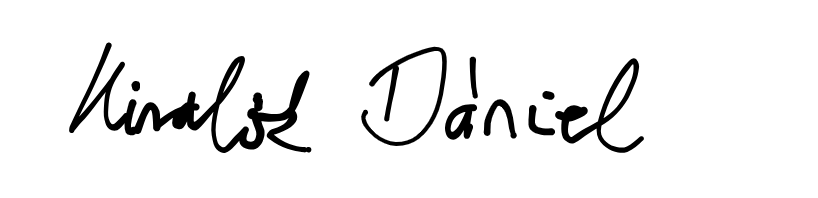
\includegraphics[width=175pt]{ alairas.png }}
\setlength{\headheight}{4em} 
\setlength{\parskip}{0.22em} 

\begin{document}
	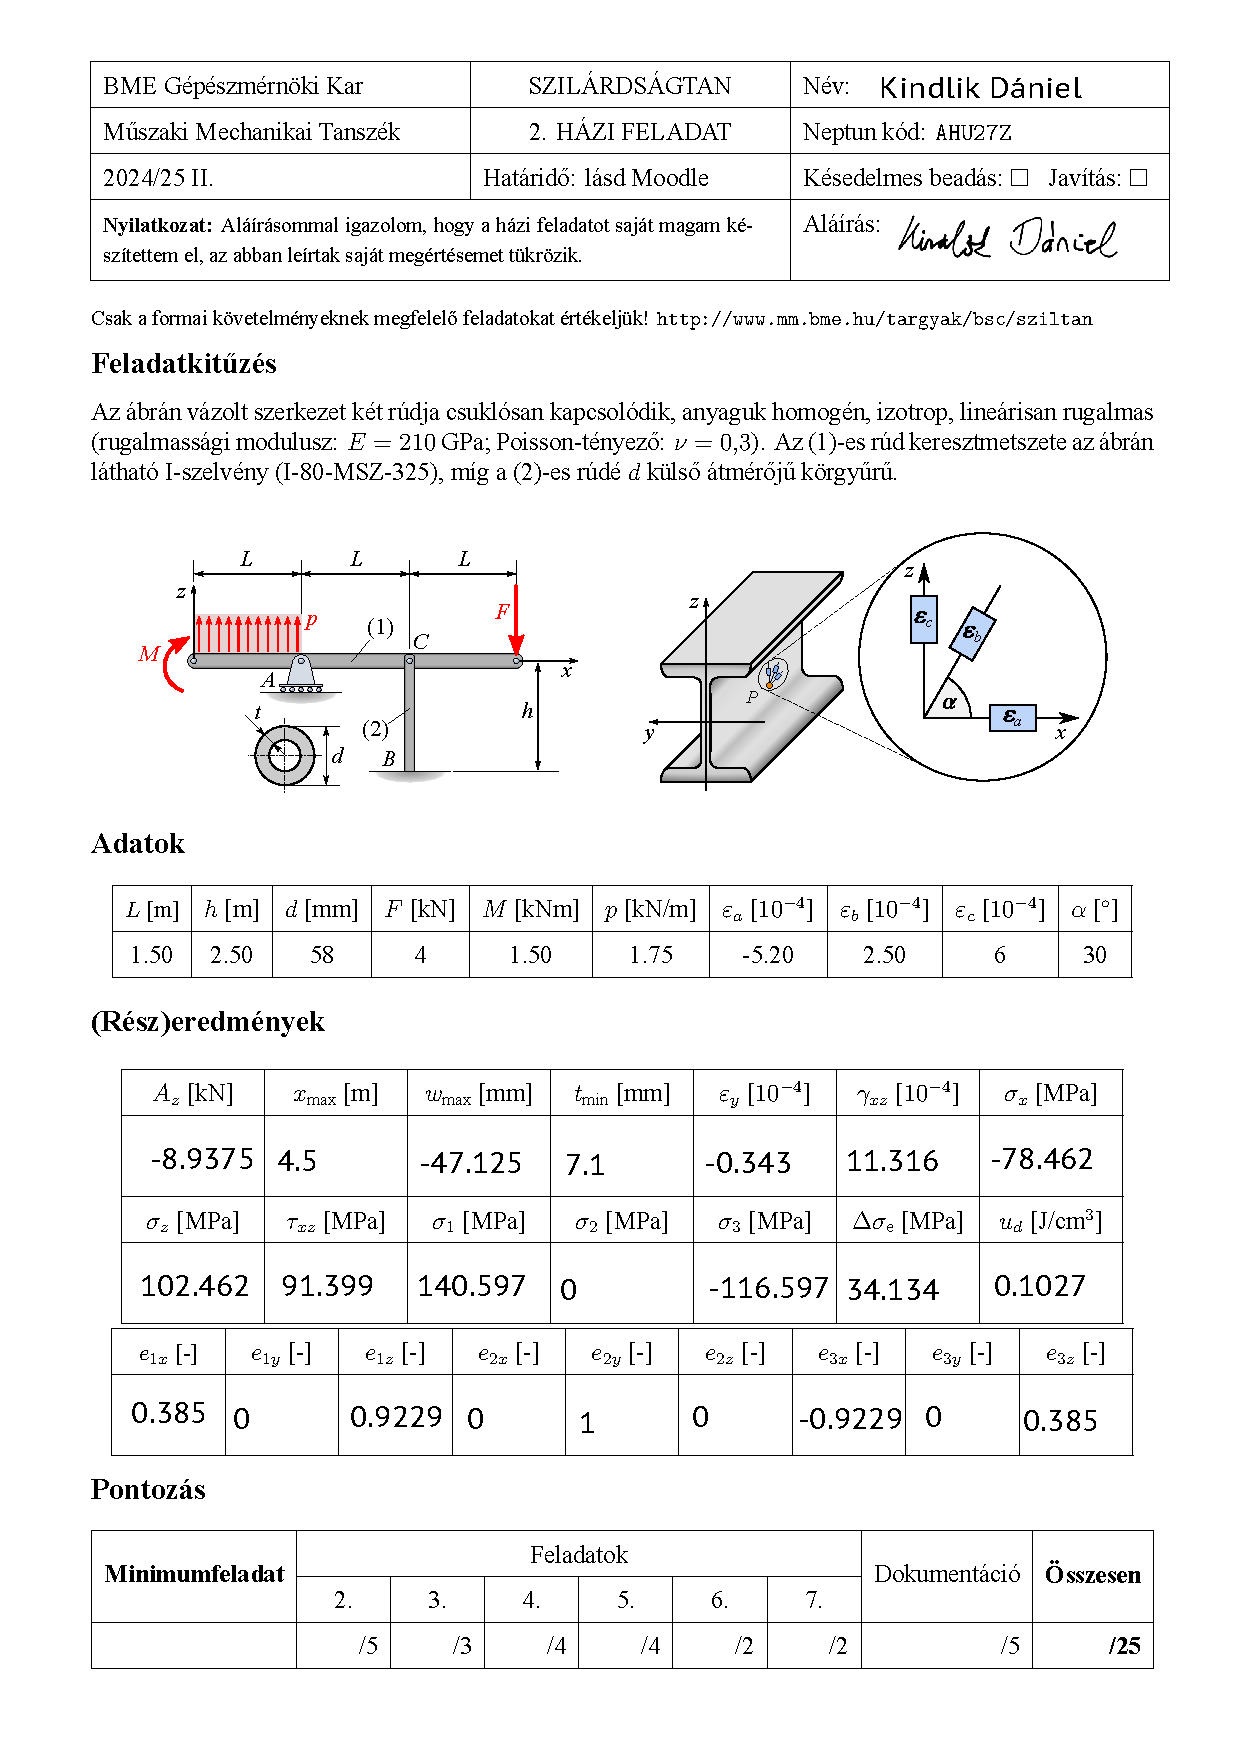
\includepdf[pages=1]{elolap.pdf}
	(A feladatokban levő egyenletrendszereket egy általam készített \textbf{Python} program segítségével oldottam meg, így azoknak csak a megoldása szerepel itt. Emellett a feladathoz szükséges ábrákat a \texttt{matplotlib} könyvtár segítségével ábrázoltam.)
	\adat
	$ L = 1.5\;\meter \;\;\;$ $ h = 2.5\;\meter \;\;\;$ $ d = 58\;\mm$\\\\
	$ F = 4\;\kn \;\;\; $ $ M = 1.5\knm $ $ p = 1.75\;\pknm \;\;\;$\\\\
	$ \varepsilon_a = -5.2\;\minegy \;\;\;$ $ \varepsilon_b = 2.5\;\minegy \;\;\;$ $ \varepsilon_c = 6\;\minegy \;\;\;$ $ \alpha = 30\;\fok \;\;\;$\\\\
	$ E = 210\;\gpa \;\;\;$ $ \nu = 0.3\;\dimnel \;\;\;$
	\setcounter{page}{1}
	\egy
	\begin{center}
		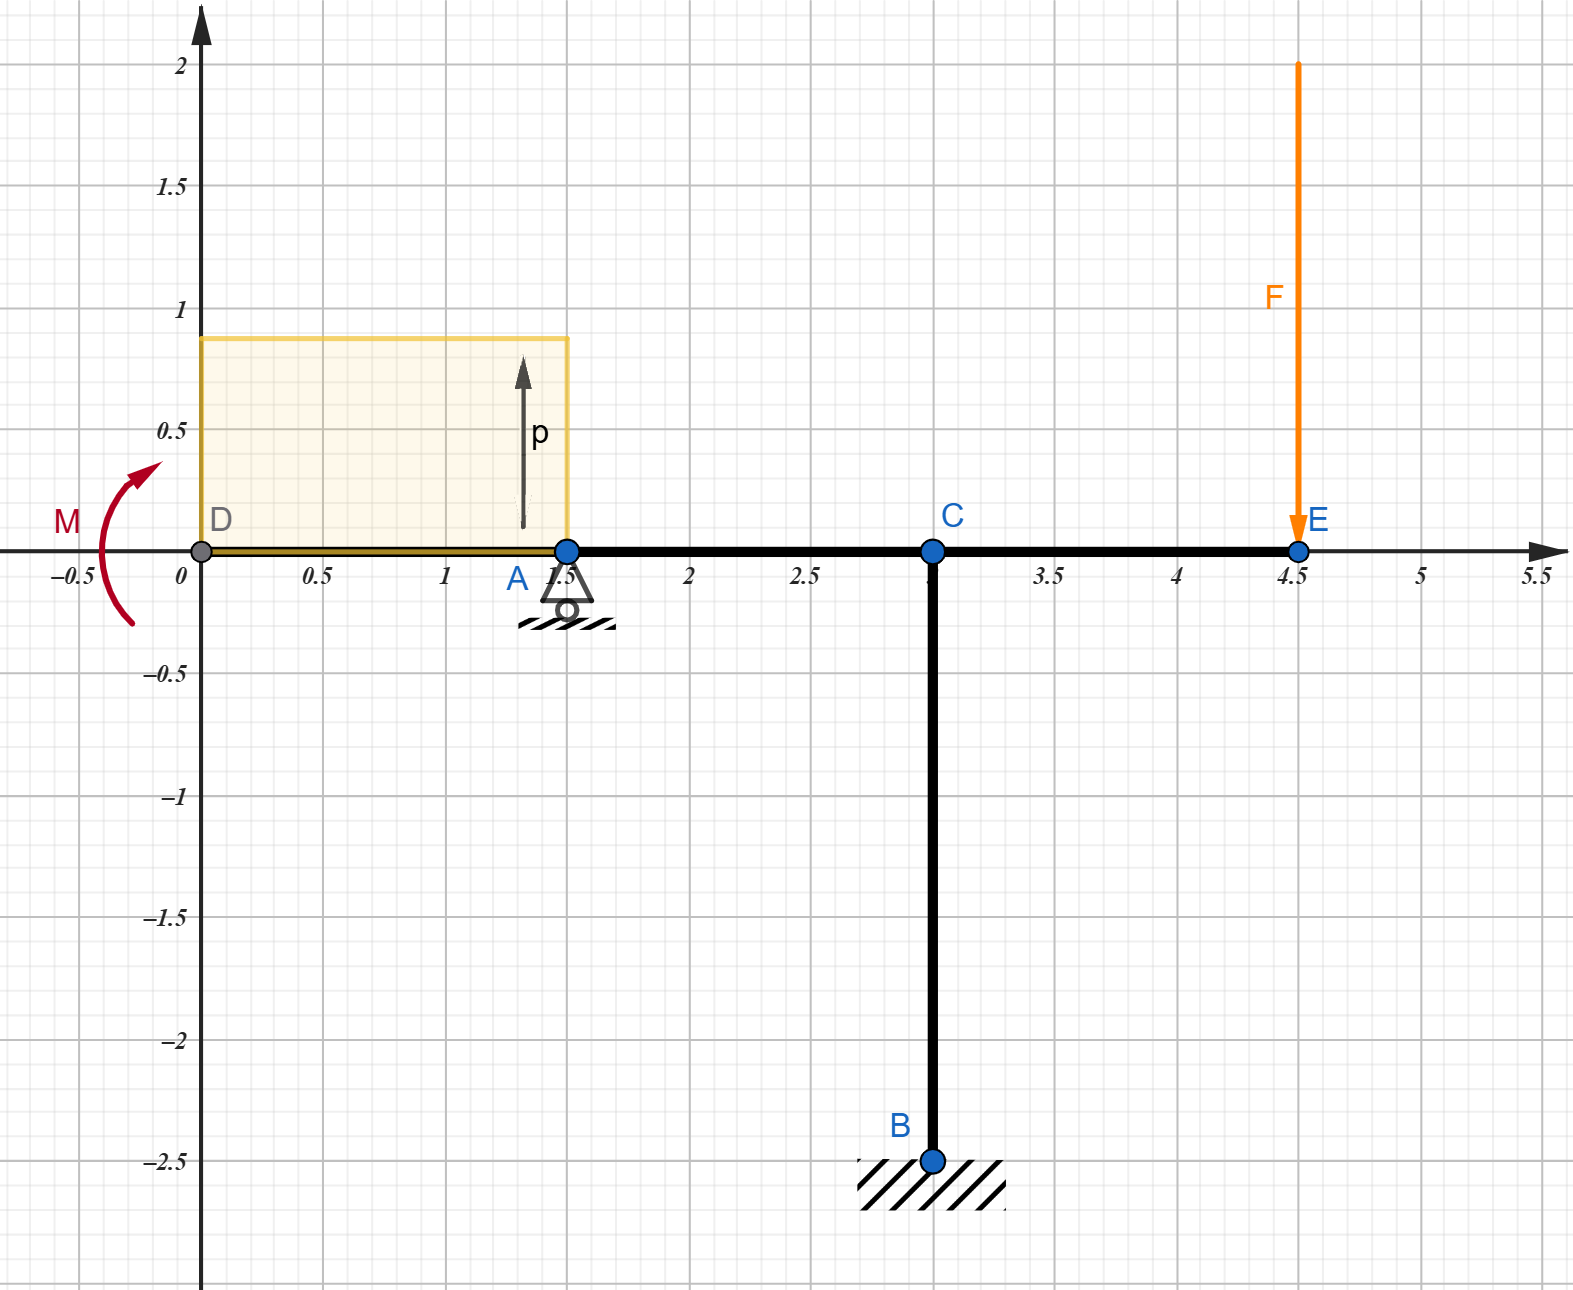
\includegraphics[width=200pt]{ meretarany.png }\\
		Az ábrán egy egység megfelel 1 m-nek és 2 kN-nak
	\end{center}
	A szerkezetünket két részre tudjuk bontani, hogy ki tudjuk számolni a reakcióerőket.\\
	Ekkor C-pontban meg fog jelenni egy C vektor, és a két rúdra külön tudunk 3-3 egyensúlyi-egyenletet írni.
	A két rész (1. eset balra, 2. eset jobbra) szabadtest-ábrája:
	\begin{center}
		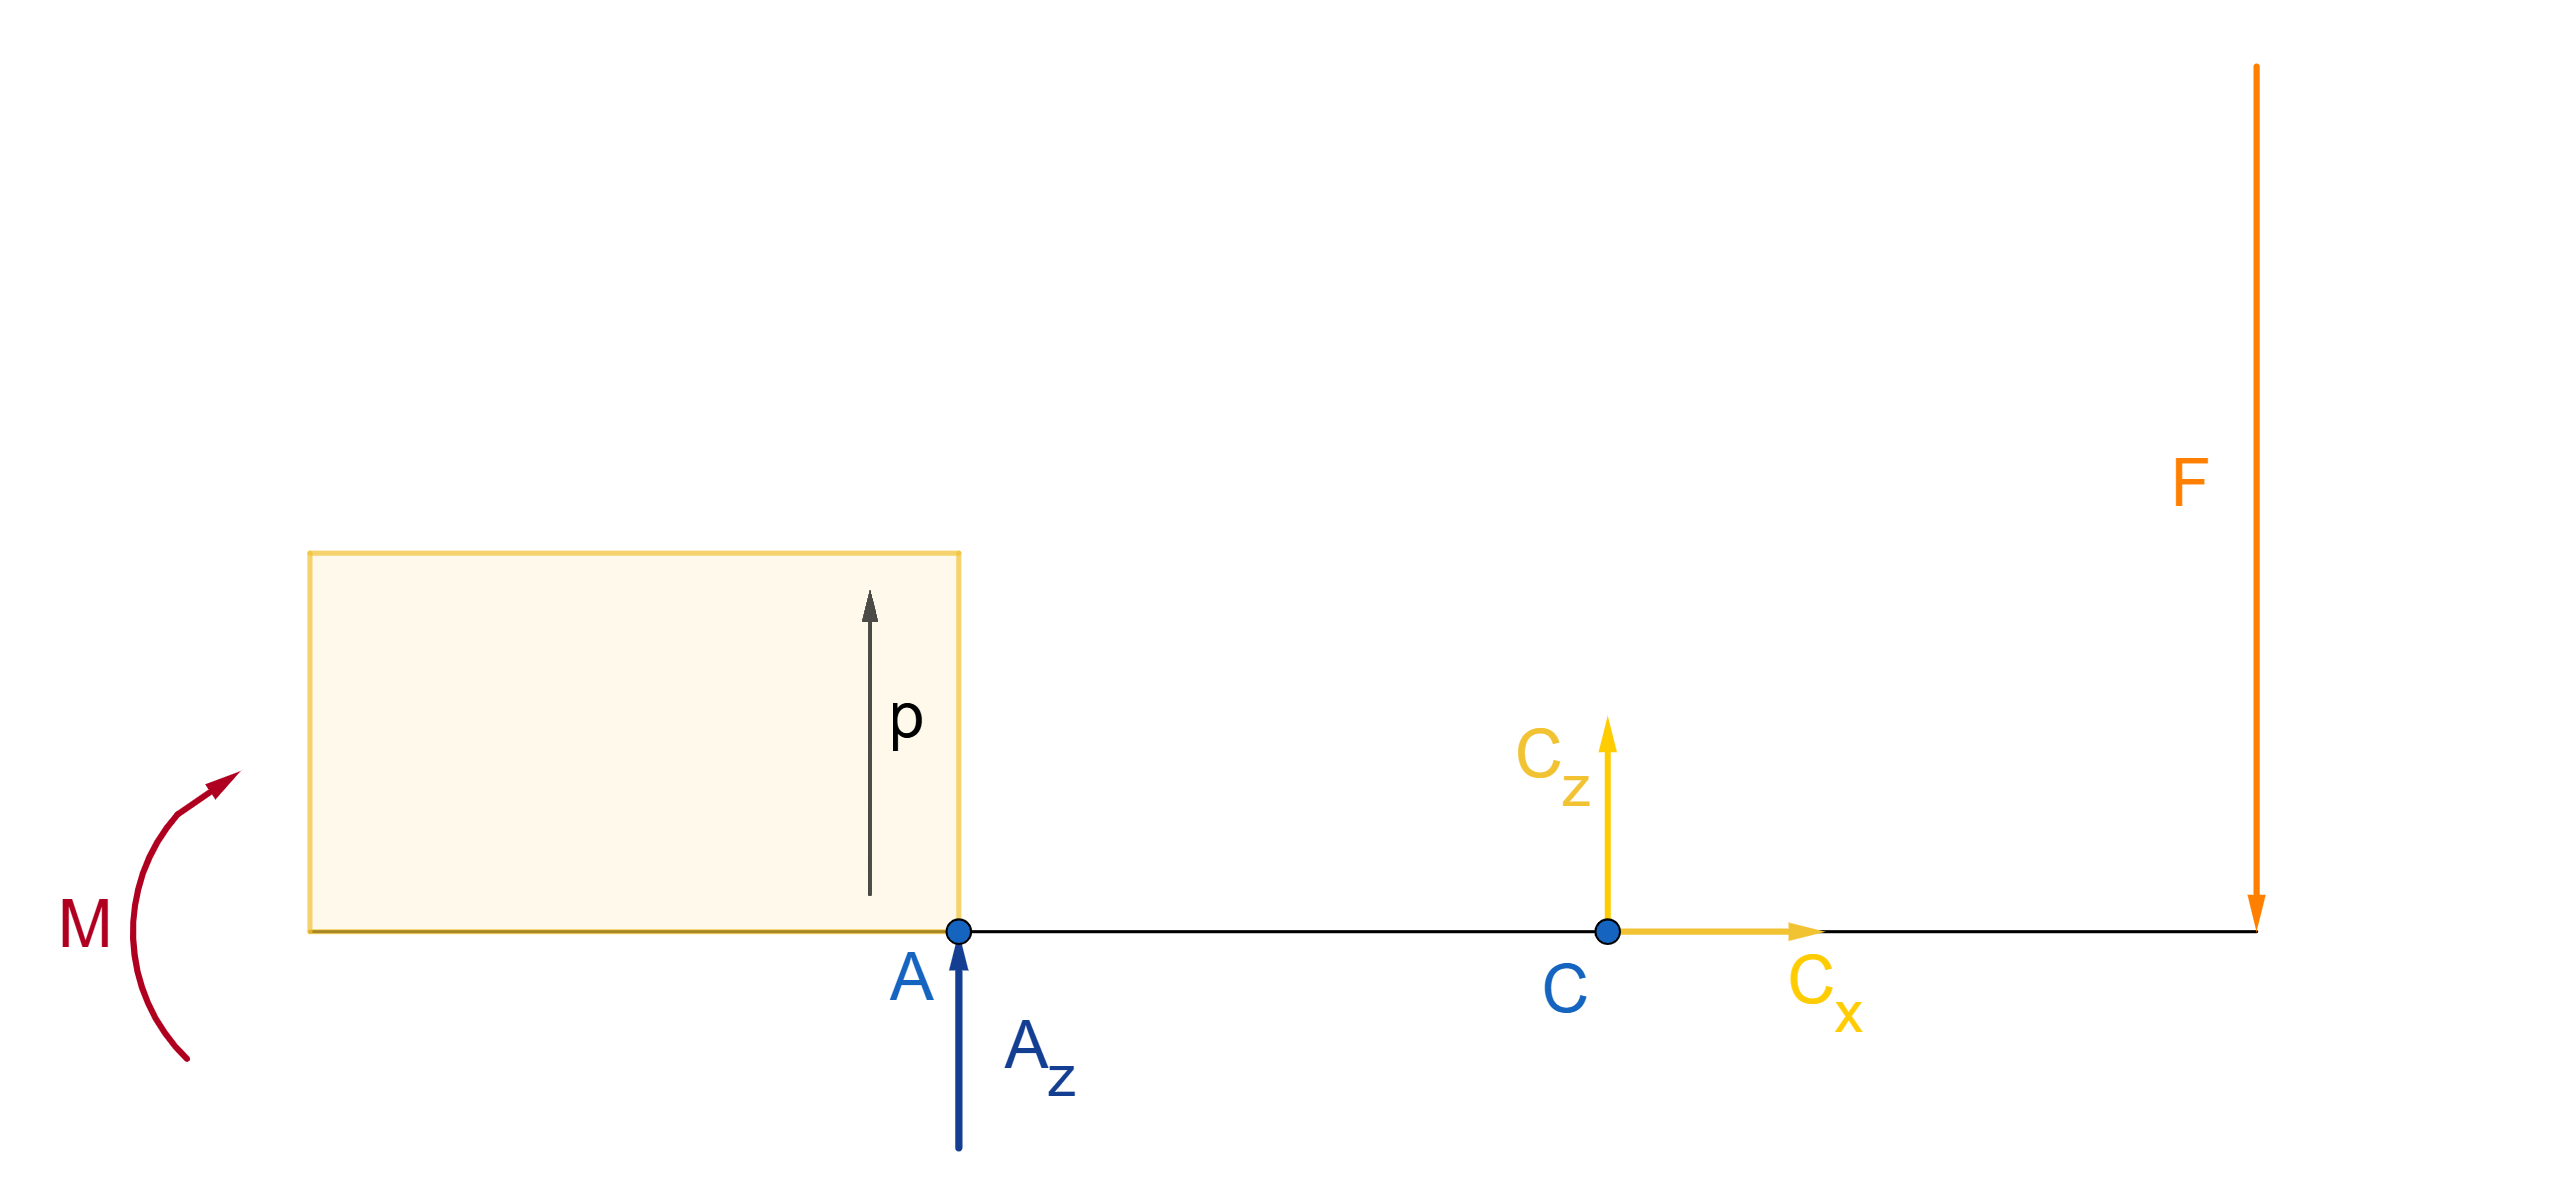
\includegraphics[width=270pt]{ SZTA1.png }
		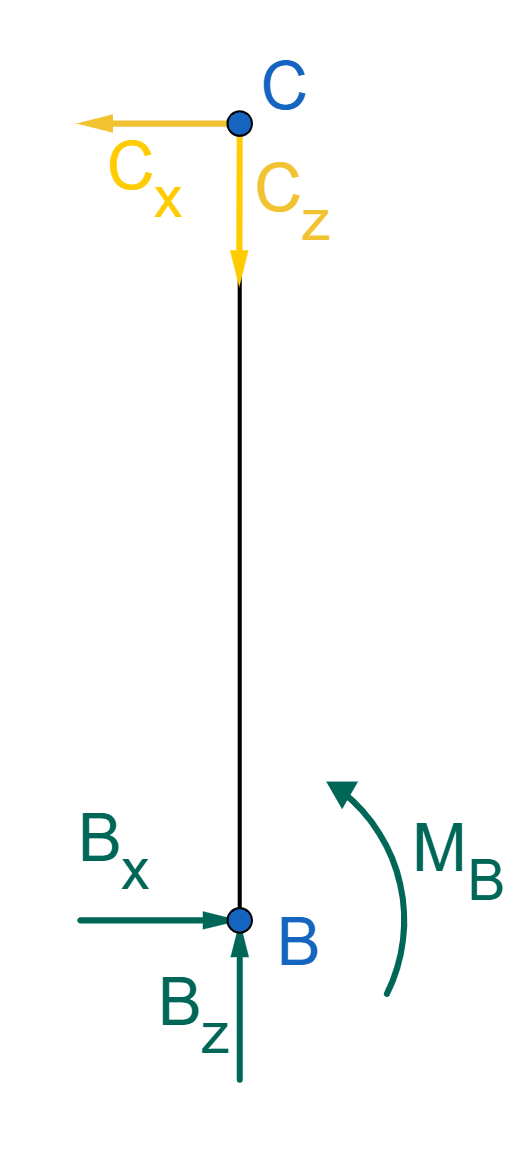
\includegraphics[width=70pt]{ SZTA2.png }
	\end{center}
	$ $
	1. esetben kijövő egyensúlyi egyenletek A pontra vonatkoztatva:\\\\
	\tabto{50pt}(1) $\sum{F_x} = 0 = C_x$\\\\
	\tabto{50pt}(2) $\sum{F_z} = 0 = A_z + C_z + p \cdot L - F$\\\\
	\tabto{50pt}(3) $\sum{M_{A}} = 0 = C_z \cdot L - M - F \cdot 2L - (p \cdot L) \cdot \frac{L}{2}$\\\\
	2. esetben kijövő egyensúlyi egyenletek B pontra vonatkoztatva:\\\\
	\tabto{50pt}(4) $\sum{F_x} = 0 = -C_x + B_x$\\\\
	\tabto{50pt}(5) $\sum{F_z} = 0 = -C_z + B_z$\\\\
	\tabto{50pt}(6) $\sum{M_B} = 0 = M_B + B_x \cdot h$\\\\
	A két egyenletrendszer megoldása:\\\\
	\tabto{50pt}$A_z = \underline{\underline{-8.9375 \kn}}$\\\\
	\tabto{50pt}$B_x = \underline{\underline{0 \kn}}$\\\\
	\tabto{50pt}$B_z = \underline{\underline{10.3125 \kn}}$\\\\
	\tabto{50pt}$M_B = \underline{\underline{0 \knm}}$\\\\
	\tabto{50pt}$C_x = \underline{\underline{0 \kn}}$\\\\
	\tabto{50pt}$C_z = \underline{\underline{10.3125 \kn}}$
	\newpage
	\ketto
	Ahhoz hogy meg tudjuk határozni w(x)-et először meg kell adnunk az (1)-es rúd hajlítónyomatéki igénybevételét. A szerkezetet három részre tudjuk bontani, így a függvény:
	\begin{table}[h]
		\renewcommand{\arraystretch}{1.8}
		\resizebox{\textwidth}{!}{%
			\centering
			\begin{tabular}{c|c|c|c}
				&\begin{tabular}[c]{@{}c@{}}I.\\ $0 < x < 1.5$\end{tabular}&
				\begin{tabular}[c]{@{}c@{}}II.\\ $1.5 < x < 3$\end{tabular}&
				\begin{tabular}[c]{@{}c@{}}III.\\ $3 < x < 4.5$\end{tabular} \\ \hline
				$ \text{M}_h$&
				\begin{tabular}[c]{@{}c@{}}$- M - p \cdot x \cdot \dfrac{x}{2} =$\\ $= -0.875x^2 - 1.5 \knm$\end{tabular}&
				\begin{tabular}[c]{@{}c@{}}$- M - p \cdot L \cdot (x - \dfrac{L}{2}) - A_z \cdot (x - L)=$\\ $= 6.315x - 12.9375 \knm$\end{tabular}&
				\begin{tabular}[c]{@{}c@{}}$- M - p \cdot L \cdot (x - \dfrac{L}{2}) - A_z \cdot (x - L) - C_z \cdot (x - 2L)=$\\ $= 18 - 4x \knm$\end{tabular} \\
			\end{tabular}%
		}
	\end{table}\\\\
	Az egyenletekből adódó függvény:
	\begin{center}
		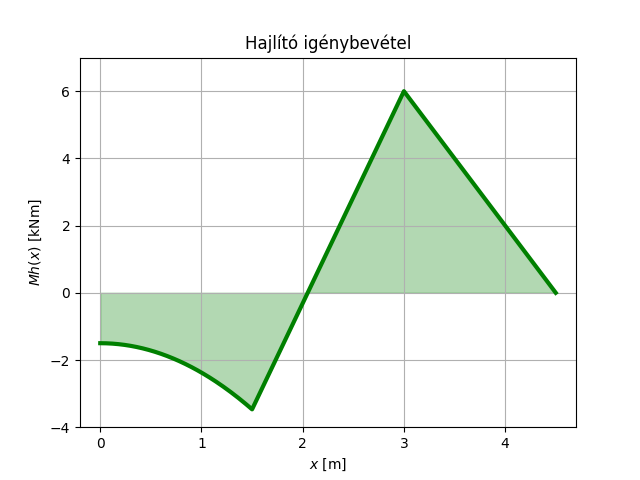
\includegraphics[width=275pt]{ hajlito.png }
	\end{center}
	Az (1)-es rúd lehajlásfüggvényének meghatározásához felhasználhatjuk az alábbi összefüggéseket:\\\\
	$-I \cdot E \cdot w''(x) = M_h(x) \xrightarrow{} -I \cdot E \cdot w'(x) = \int M_h(x) \xrightarrow{} -I \cdot E \cdot w(x) = \iint M_h(x)$\\\\
	Ezek az összefüggések a rúd egészén igazak, úgyhogy felírom a hajlítónyomaték-függvény három szakaszának szükséges alakjait:
		\begin{table}[h]
		\renewcommand{\arraystretch}{1.8}
		\resizebox{\textwidth}{!}{%
			\centering
			\begin{tabular}{c|c|c|c}
				&I. ($w''_1(x),  w'_1(x),  w_1(x)$)&II. ($w''_2(x),  w'_2(x),  w_2(x)$)&III. ($w''_3(x),  w'_3(x),  w_3(x)$)\\ \hline
				$ M_h(x)$&
				$-0.875x^2 - 1.5$&
				$6.315x - 12.9375$&
				$18-4x$ \\ \hline
				$ \int M_h(x)$&
				$-0.2917x^3 - 1.5x + C_{11}$&
				$3.15625x^2 - 12.9375x + C_{21}$&
				$-2x^2 + 18x + C_{31}$ \\ \hline
				$ \iint M_h(x)$&
				$-0.072917x^4 - 0.75x^2 + C_{11}x + C_{12}$&
				$1.052083x^3 - 6.46875x^2 + C_{21}x + C_{22}$&
				$-0.667x^3 + 9x^2 + C_{31}x + C_{32}$\\
			\end{tabular}%
		}
	\end{table}\\
	Az egyenletekben az integrálás miatt megjelenő ismeretleneket a peremfeltételekből kijövő egyenletrendszerrel tudjuk kiszámolni, itt elhagyhatjuk a $-I \cdot E$ szorzót.\\\\
	A peremfeltételek:\\\\
	$w_1(L) = 0 \quad w_2(L) = 0 \quad w_2(2L) = 0 \quad w_3(2L) = 0 \quad w'_1(L) = w'_2(L) \quad w'_2(2L) = w'_3(2L)$\\\\
	Ezek alapján be tudunk helyettesíteni az x-ek helyére számokat, és 6db egyenletünk jön ki.\\\\\\
	Az egyenletrendszer megoldása:\\\\
	$C_{11} = 3.4688 \;\; C_{12} = -3.1465 \;\; C_{21} = 12.539 \;\; C_{22} = -7.8047 \;\; C_{31} = -33.8672 \;\; C_{32} = 38.6016$\\\\
	Az így kijövő eredményeket fel tudjuk használni $w(x)$ és $\varphi(x)$függvény meghatározásához:\\\\
	$w(x) = -\dfrac{1}{I \cdot E} \cdot \iint M_h(x) \quad\quad \varphi(x) = -\dfrac{1}{I \cdot E} \cdot \int M_h(x)$
		\begin{table}[h]
		\renewcommand{\arraystretch}{1.8}
		\resizebox{\textwidth}{!}{%
			\centering
			\begin{tabular}{c|c|c|c}
				&\begin{tabular}[c]{@{}c@{}}I.\\ $0 < x < 1.5$\end{tabular}&
				\begin{tabular}[c]{@{}c@{}}II.\\ $1.5 < x < 3$\end{tabular}&
				\begin{tabular}[c]{@{}c@{}}III.\\ $3 < x < 4.5$\end{tabular} \\ \hline
				$ w(x)$&
				$0.446x^4 + 4.59x^2 - 21.231x + 19.259$&
				$-6.439x^3 + 39.593x^2 - 76.748x + 47.77$&
				$4.08x^3 - 55.0863x^2 + 207.2909x - 236.269$ \\ \hline
				$ \varphi(x)$&
				$1.785x^3 + 9.181x - 21.2312$&
				$-19.318x^2 + 79.187x - 76.748$&
				$12.2414x^2 - 110.173x + 207.291$ \\
			\end{tabular}%
		}
	\end{table}
	\begin{center}
		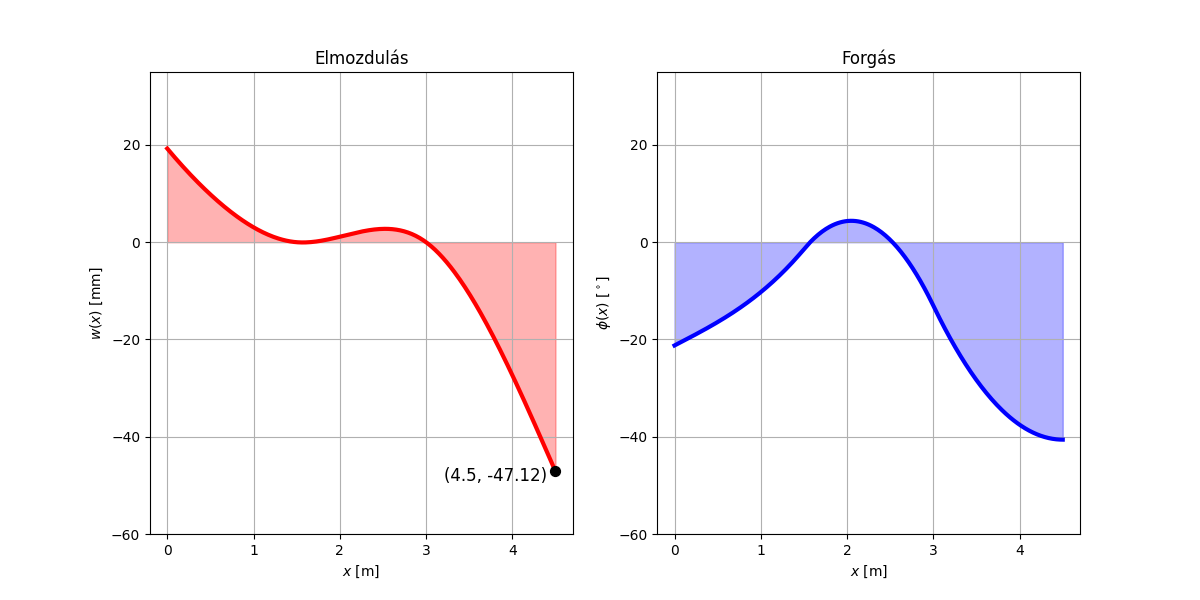
\includegraphics[width=450pt]{ elmforg.png }
	\end{center}
	Az ábráról láthatjuk, hogy a legnagyobb lehajlás $x = 4.5$-nél következik be:\\\\
	$x_{max} = \underline{\underline{4.5 \meter}} \quad w_{max} = w(4.5) = \underline{\underline{-47.12 \mm}}$
	\newpage
	\harom
	$\sigma_F = 240 \mpa \quad \lambda_0 = 105 \quad \sigma_{kr}=308 - 1.14\lambda$\\\\
	A $\sigma - \lambda$ diagram 3 részből fog állni: Folyáshatár, Tetmajer-egyenes és Euler-hiperbola\\\\
	A diagram ábrázolásához meg kell adnunk a folyáshatár és Tetmajer-egyenes váltópontját, valamint az Euler-hiperbola egyenletét:\\\\
	$ 240 = 308 - 1.14\lambda_F \xrightarrow{} \lambda_F = 59.65$\\\\
	Euler-hiperbola egyenlete: $\left( \dfrac{\pi}{\lambda} \right)^2 \cdot 2E$
	\begin{center}
		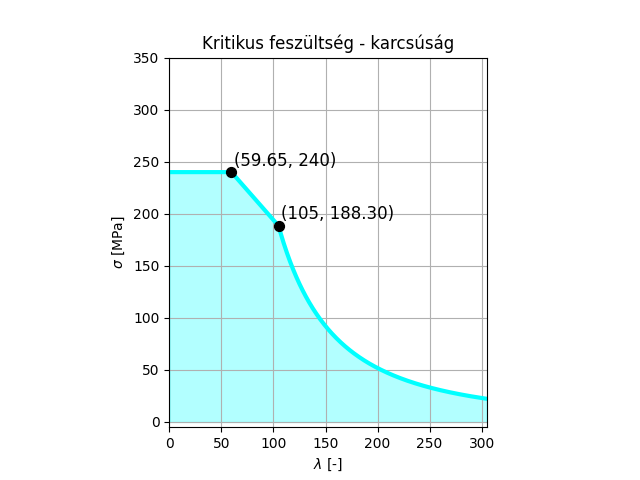
\includegraphics[width=265pt]{ krfesz.png }
	\end{center}
	A méretezés elvégzéséhez tegyük fel, hogy az Euler-tartományban vagyunk:
	\begin{center}
		$F_t = \left( \dfrac{\pi}{c \cdot L} \right)^2 \cdot I_2 \cdot E$
	\end{center} 
	$F_t = 3 \cdot |C_z|$ mivel háromszoros biztonságot akarunk\\\\
	$c = 2$ mivel alul be van fogva a rúd, felül pedig szabadon mozoghat\\\\
	$I_2 = \dfrac{(d^4 - (d-2t)^4) \cdot \pi}{64}$ mivel körgyűrűről beszélünk\\\\
	Az egyenleteket összevonva és átrendezve: $t_{min} = \underline{\underline{7.05 \approx 7.1 \mm}}$\\\\
	Így $\lambda$ karcsúság értéke:
	\begin{center}
		$\lambda = \dfrac{L_0}{i_2} = \dfrac{c \cdot L}{\sqrt[]{\dfrac{I_2}{A}}}$
	\end{center}
	Ezek alapján $\lambda = \underline{\underline{275.1774}} > \lambda_0$, tehát helyes volt a feltételezésünk
	\negy
	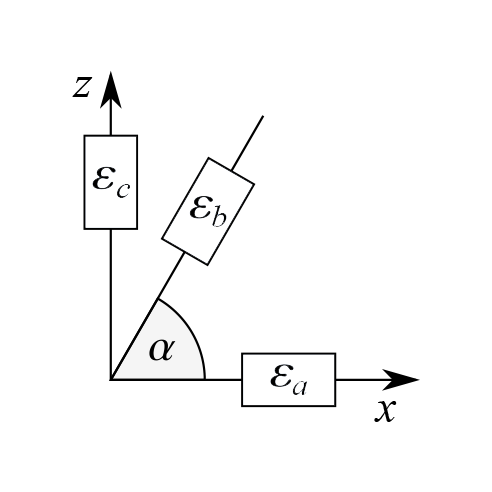
\includegraphics[width=80pt]{epsilonabra.png}\\
	A nyúlásmérő-bélyegek elhelyezkedése miatt célszerű nevezések: $\varepsilon_x = \varepsilon_a \text{ és } \varepsilon_z = \varepsilon_c$\\\\
	$\varepsilon_y \text{ és } \gamma_{xz}$ megadására ezek alapján használhatunk két egyenletet:\\\\
	$\varepsilon_b = \varepsilon_a \cdot \cos[2](\alpha) + \varepsilon_b \cdot \sin[2](\alpha) + \dfrac{\gamma_{xz}}{2} \cdot \sin(2\alpha) \xrightarrow{} \gamma_{xz} = 11.316 \minegy$\\\\
	$\varepsilon_y = -\dfrac{\nu \cdot (\varepsilon_x + \varepsilon_z)}{1 - \nu} \xrightarrow{} \varepsilon_y = -0.343 \minegy$\\\\
	Ezek alapján az alakváltozási tenzor: $\boldsymbol{\varepsilon} = 
	\begin{bmatrix}
		\varepsilon_x & 0 & \frac{1}{2}\gamma_{xz}\\
		0 & \varepsilon_y & 0\\
		\frac{1}{2}\gamma_{xz} & 0 & \varepsilon_z
	\end{bmatrix} = 
	\underline{\underline{\begin{bmatrix}
	-5.2 & 0 & 5.658\\
	0 & -0.343 & 0\\
	5.658 & 0 & 6
	\end{bmatrix} \minegy}}$\\\\
	A Hooke-törvény segítségével meg tudjuk adni a feszültségi tenzort:
	\begin{center}
		$\boldsymbol{\sigma} = \dfrac{E}{1 + \nu} \cdot \left( \boldsymbol{\varepsilon} + \dfrac{\nu}{1 - 2\nu} \cdot \varepsilon_1 \cdot \textbf{E} \right)$
	\end{center}
	$\varepsilon_1 = \dfrac{\Delta V}{V} = tr(\boldsymbol{\varepsilon}) = \varepsilon_x + \varepsilon_y + \varepsilon_z = \underline{\underline{0.457 \minegy}}$\\\\
	Ezek alapján az feszültségi tenzor: $\boldsymbol{\sigma} = 
	\begin{bmatrix}
		\sigma_x & 0 & \tau_{xz}\\
		0 & \sigma_y & 0\\
		\tau_{xz} & 0 & \sigma_z
	\end{bmatrix} = 
	\underline{\underline{\begin{bmatrix}
		-78.462 & 0 & 91.399\\
		0 & 0 & 0\\
		91.399 & 0 & 102.462
	\end{bmatrix} \mpa}}$\\\\
	$\sigma_I = tr(\boldsymbol{\sigma}) = \underline{\underline{24 \mpa}}$\\\\
	$\sigma_{II} = \sigma_x \cdot \sigma_z - \tau^2_{xz} = \underline{\underline{-16393 \left[\text{MPa}^2\right]}}$\\\\
	$\sigma_{III} = det(\boldsymbol{\sigma}) = \underline{\underline{0}}$
	\begin{center}
		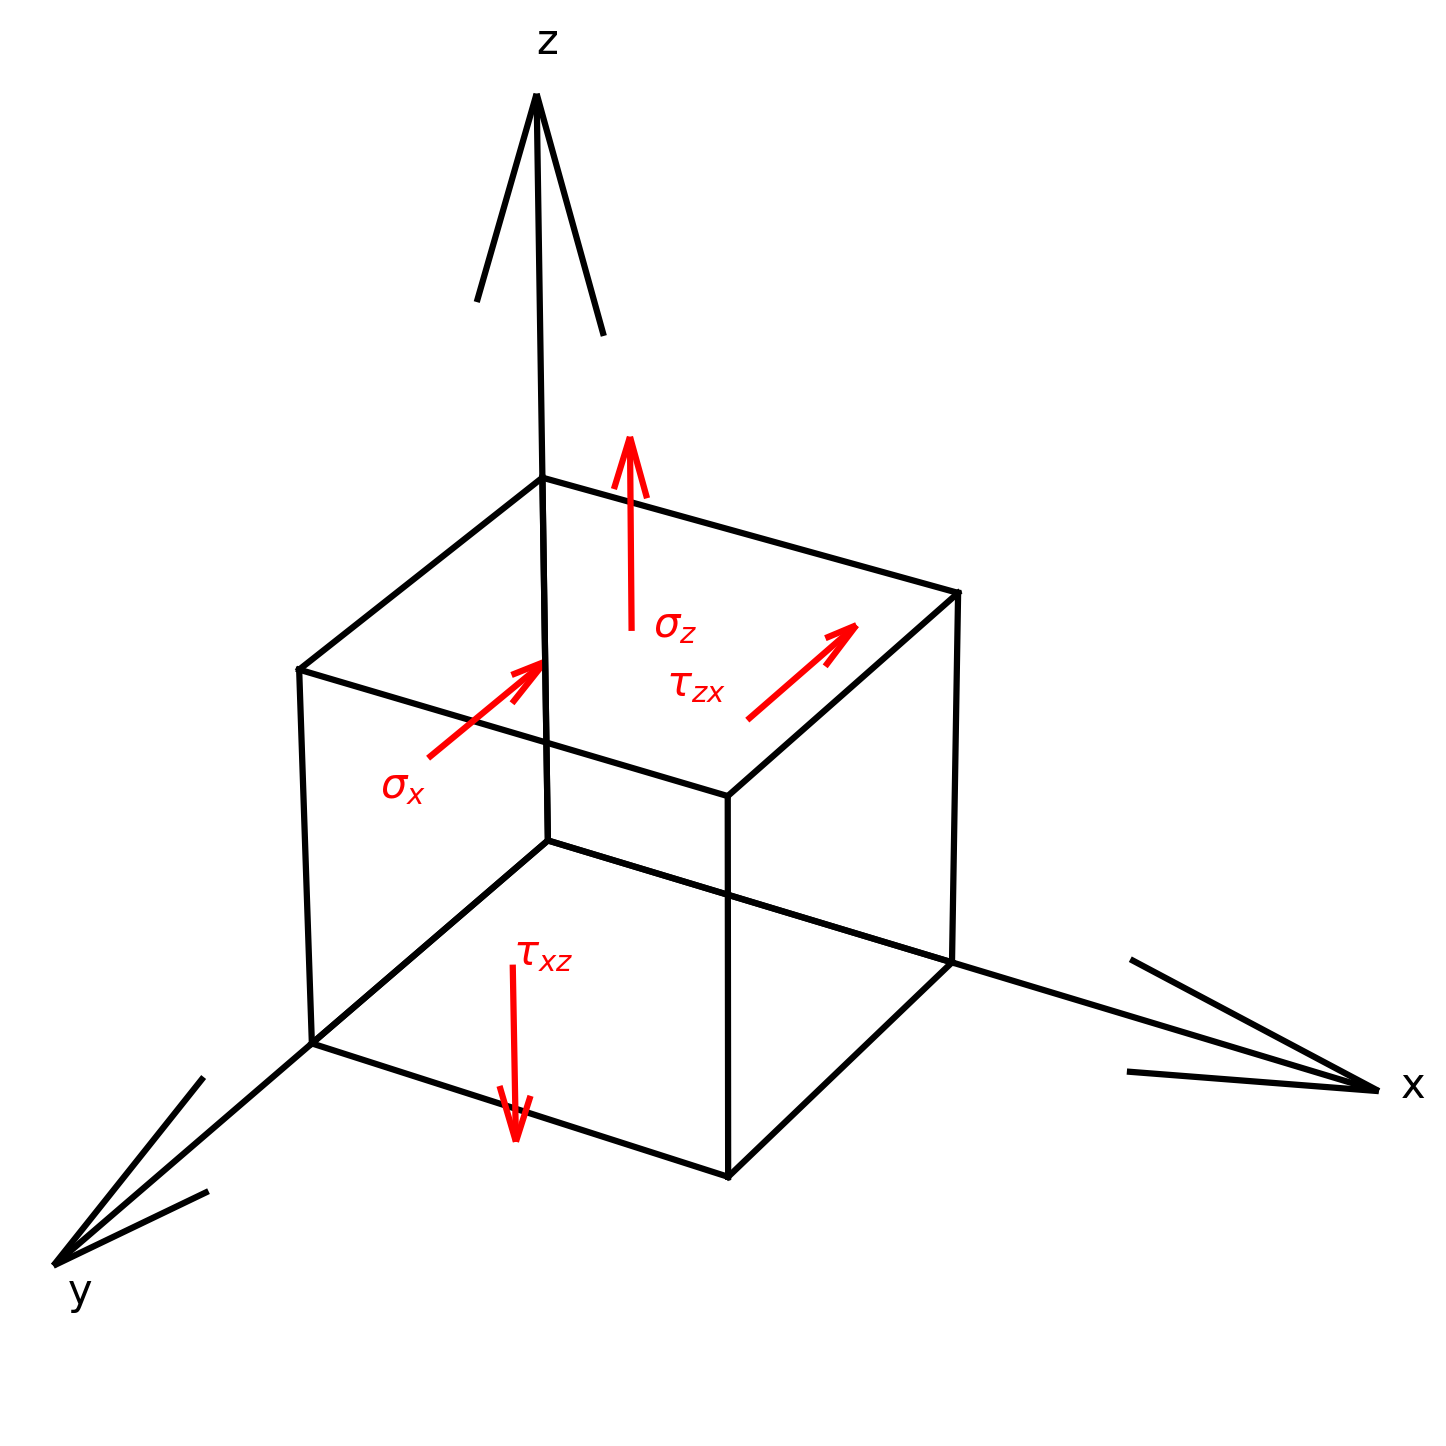
\includegraphics[width=157pt]{ kocka.png }
	\end{center}
	\ot
	$\boldsymbol{\sigma}$ mátrixból láthatjuk, hogy $\underline{e}_2$ főirány és $Y$ pont ismert.\\\\
	Mohr-körök segítségével meg tudjuk adni $\sigma_{1,2}$-t is:\\\\
	$\sigma_K = \dfrac{\sigma_x + \sigma_y}{2} \quad$
	$R = \sqrt{\left(\dfrac{\sigma_x - \sigma_y}{2}\right)^2 + \tau^2_{xz}}$\\\\
	$X(\sigma_x,\tau_{xz}) \quad Y(\sigma_y, 0) \quad Z(\sigma_z, \tau_{xz})$\\
	\begin{center}
		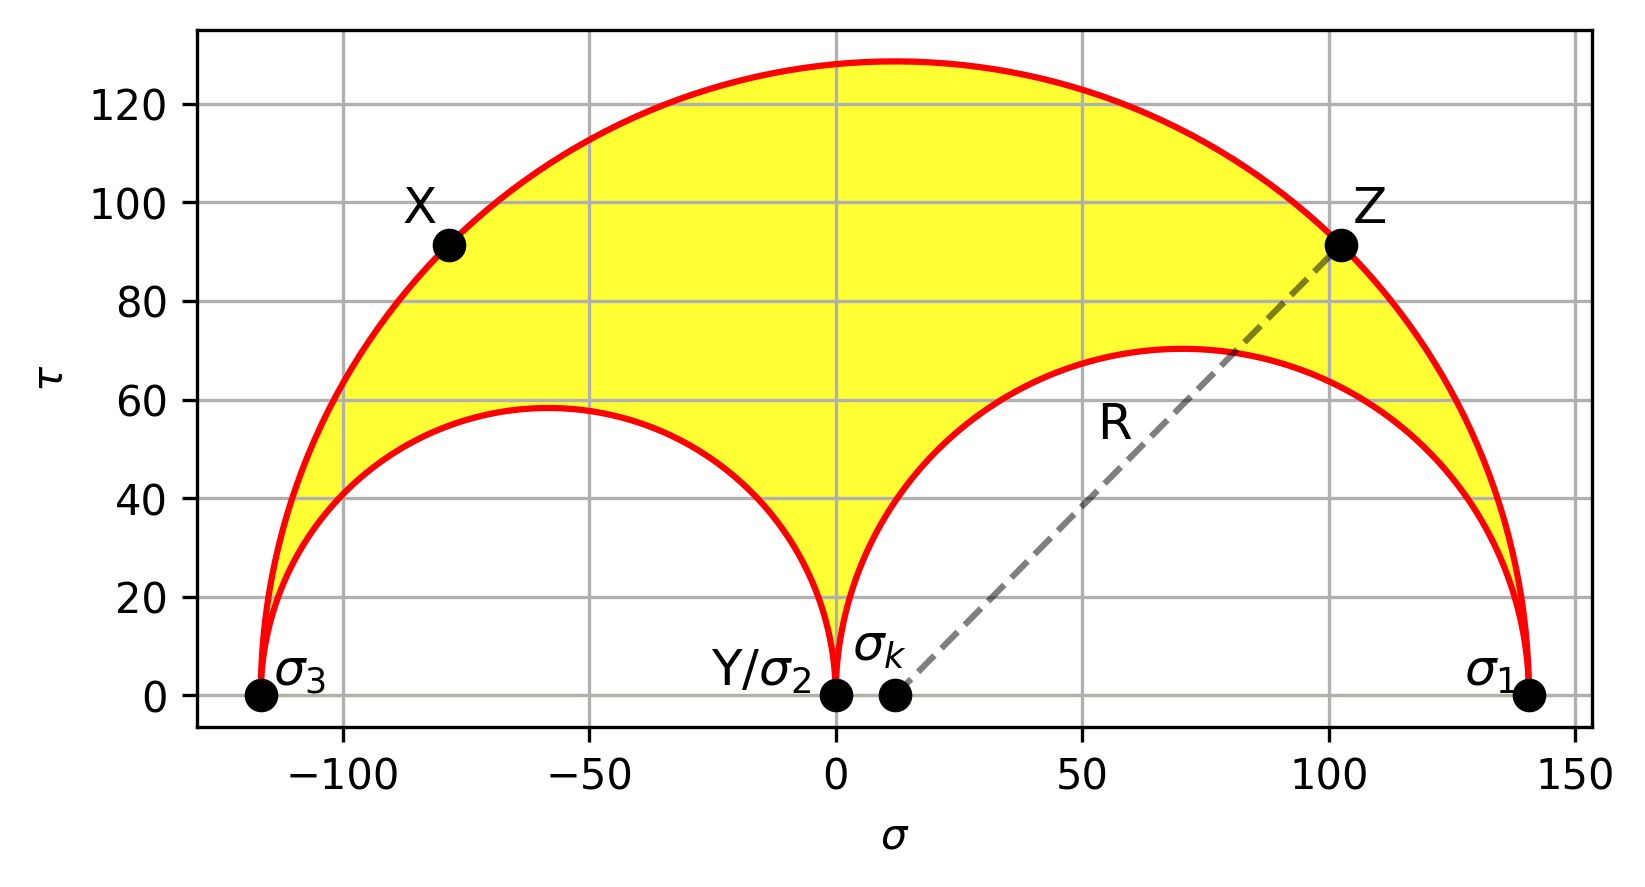
\includegraphics[width=250pt]{ Mohr.png }
	\end{center}
	Az ábra segítségével:\\\\
	$\sigma_1 = \sigma_K + R = \underline{\underline{140.597 \mpa}}$\\\\
	$\sigma_2 = \underline{\underline{0 \mpa}}$\\\\
	$\sigma_3 = \sigma_K - R = \underline{\underline{-116.597 \mpa}}$\\\\
	Az 1-es főfeszültséghez tartozó főirány: $\varphi_1 = \atan(\dfrac{\sigma_1 - \sigma_x}{\tau_{xz}}) \xrightarrow{} \underline{e}_1 = \begin{bmatrix}\cos(\varphi_1) \\ 0 \\ \sin(\varphi_1)\end{bmatrix} = \underline{\underline{\begin{bmatrix}0.385 \\ 0 \\ 0.923\end{bmatrix}}}$\\\\\\
	Az 2-es főfeszültséghez tartozó főirány ismert: $\underline{e}_2 = \underline{\underline{\begin{bmatrix}0 \\ 1 \\ 0\end{bmatrix}}}$ \\\\\\
	Az 3-as főfeszültséghez tartozó főirány:
	$\underline{e}_3 = \underline{e}_1 \times \underline{e}_2 = \underline{\underline{\begin{bmatrix}-0.9223 \\ 0 \\ 0.385\end{bmatrix}}}$
	\newpage
	\ellenorzes
	Ellenőrhetünk sajátérték-sajátvektor számítással:\\\\
	Sajátértékek:\\\\
	$det(\boldsymbol{\sigma} - \lambda \cdot \textbf{E}) = det\left(\begin{bmatrix}
		-78.462-\lambda & 0 & 91.399\\
		0 & -\lambda & 0\\
		91.399 & 0 & 102.462-\lambda
	\end{bmatrix}\right) =$\\\\ $= (-78.462-\lambda) \cdot (-\lambda) \cdot (102.462-\lambda) - (91.399) \cdot (-\lambda) \cdot (91.399) = 0$\\\\
	$\lambda_3 = -116.597\checkmark \quad \lambda_2 = 0\checkmark \quad \lambda_1 = 140.597\checkmark$\\\\
	Sajátvektorok:\\\\
	$\begin{bmatrix}
		-78.462-\lambda_{1,2,3} & 0 & 91.399\\
		0 & -\lambda_{1,2,3} & 0\\
		91.399 & 0 & 102.462-\lambda_{1,2,3}
	\end{bmatrix} \cdot \underline{e}_{1,2,3} = \begin{bmatrix}
	0\\
	0\\ 
	0 
	\end{bmatrix}$\\\\\\
	$\underline{e}_1 = \begin{bmatrix}0.385 \\ 0 \\ 0.923\end{bmatrix}\checkmark \quad \underline{e}_2 = \begin{bmatrix}0 \\ 1 \\ 0\end{bmatrix}\checkmark \quad \underline{e}_3 = \begin{bmatrix}-0.9223 \\ 0 \\ 0.385\end{bmatrix}\checkmark$
	\hatodik
	Mohr-féle egyenértékű feszültség: $\sigma_e^{Mohr} = \sigma_1 - \sigma_3 = \underline{\underline{257.193 \mpa}}$\\\\
	HMH-féle egyenértékű feszültség: $\sigma_e^{HMH} = \sqrt{\dfrac{(\sigma_1 - \sigma_2)^2 + (\sigma_2 - \sigma_3)^2 + (\sigma_3 - \sigma_1)^2}{2}} = \underline{\underline{223.059 \mpa}}$\\\\
	A kettő különbsége: $\Delta\sigma_e = \sigma_e^{Mohr} - \sigma_e^{HMH} = \underline{\underline{34.134 \mpa}}$
	\het
	Alakváltozási energiasűrűség értéke:\\\\
	$u = \dfrac{\boldsymbol{\sigma} : \boldsymbol{\varepsilon}}{2} = \dfrac{\sigma_x \cdot \varepsilon_x + \tau_{xz} \cdot \gamma_{xz} + \sigma_z \cdot \varepsilon_z}{2} = \underline{\underline{0.10285 \jpcm}}$\\\\
	Térfogatváltozásra forduló komponens:\\\\
	$u_h =  \dfrac{\left(\dfrac{1}{3}tr(\boldsymbol{\sigma}) \cdot \textbf{E})\right) : \left(\dfrac{1}{3}tr(\boldsymbol{\varepsilon}) \cdot \textbf{E}\right)}{2}= \dfrac{1}{6}\sigma_1 \cdot \varepsilon_1 = \underline{\underline{1.82857 \cdot 10^{-4} \jpcm}}$\\\\
	Ezek alapján az alaktorzulásra forduló komponens:\\\\
	$u_d = u - u_h = \underline{\underline{0.10267 \jpcm}}$
\end{document}